%% LyX 2.0.8.1 created this file.  For more info, see http://www.lyx.org/.
%% Do not edit unless you really know what you are doing.
\documentclass[english]{article}
\usepackage[T1]{fontenc}
\usepackage[utf8]{luainputenc}
\usepackage{array}
\usepackage{multirow}
\usepackage{graphicx}

\makeatletter

%%%%%%%%%%%%%%%%%%%%%%%%%%%%%% LyX specific LaTeX commands.
%% Because html converters don't know tabularnewline
\providecommand{\tabularnewline}{\\}

%%%%%%%%%%%%%%%%%%%%%%%%%%%%%% User specified LaTeX commands.
\usepackage{cite}
\usepackage[T1]{fontenc}
\usepackage{inputenc}
\usepackage{authblk}

\makeatother

\usepackage{babel}
\begin{document}

\title{Estimating Drivers Cell State Transitions using Gene Regulatory Network
Models\author[1]{Daniel Schlauch} 
\author[2,3]{Kimberly Glass} 
\author[1,3]{John Quackenbush} 
\affil[1]{Department of Biostatistics and Computational Biology, Dana-Farber Cancer Institute and Department of Biostatistics, Harvard TH Chan School of Public Health, Boston, MA 02215}
\affil[2]{Channing Division of Network Medicine, Brigham and Women's Hospital, Boston, MA 20015}
\affil[3]{Department of Medicine, Harvard Medical School, Boston, MA 20015}}
\maketitle
\begin{abstract}
Abstract In the language of systems biology, the state of a cell can
be represented by a gene regulatory network that characterizes the
gene transcriptional processes that are active in that cell type.
And transitions that occur in a wide range of biological processes,
ranging from development to disease, can be thought of as transformation
of the gene regulatory network from its initial state to its final
state. Here we propose a regression-based generalization of the PANDA
method for gene regulatory network inference for individual states,
and a linear algebra approach to modeling cell state transitions,
identifying transcription factors that alter the network structure
as cell states change.
\end{abstract}

\section*{The problem of gene regulatory network inference }

One of the fundamental problems is biology is modeling the transition
between biological states such as that which occurs during development
or as a healthy tissue transforms into a disease state. While it is
appealing to conceive of this process as deterministic, reflecting
a change from one well-defined phenotype to another, in truth the
situation is much more complex. Neither the initial nor the final
phenotype is discrete, but each falls into a continuum of states,
which, on average, captures features of that phenotype. Indeed, within
each tissue there are many, many cells, each of which is its own particular
instance of that tissue—with unique patterns of gene expression and
individual regulatory processes. The same is true when considering
individuals as each healthy and disease state is unique to each member
of a study population. One way to conceptualize the state transition
problem is to imagine that each phenotype has a characteristic gene
regulatory network and that there are a set of processes that are
either activated or inactivated to transform the network in the initial
state into that characterizing the final state. Identifying those
changes could, in principle, help us to understand not only the processes
that drive the state change, but also how one might intervene to either
promote or inhibit such a transition.

As our ability to generate large-scale, integrative multi-omic datasets
has grown, there has been an increased interest in using those data
to infer gene regulatory networks to model fundamental biological
processes. While there have been many network inference methods published,
each of which uses a different approach to estimating the “strength”
of interactions between genes (or between transcription factors and
their targets), they all suffer from the same fundamental limitation.
Every method relies on estimating weights that represent the likelihood
of an interaction between two genes and then setting a threshold to
identify “real” (high confidence) edges. While setting edge confidence
thresholds allows us to graphically represent networks and allows
us to compare networks based on the presence or absence of edges,
it ultimately requires that we discard information regarding those
“weak” edges that fail to reach significance. Now, one could argue
that discarding low significance edges is sensible as one common goal
in network inference is to deduce a single, high confidence network
model that represents a particular phenotype under study or, in some
cases, a transition between phenotypes. An alternative view is that
these edges contain estimates for gene coexpression that may be muted
due to the heterogeneity of the biological sample and that networks
are best described by edgeweights on a continuous scale. Furthermore,
we argue that the inclusion of all network edgeweights in downstream
analyses allows for the collection of systematic, though subtle, differences
in coexpression which may otherwise have been washed out by extraneous
noise.


\section*{BERE: A regression-based approach to modeling gene regulatory networks }

In 2013, we described PANDA~\cite{glass2013passing}, a method~\cite{olsen2014inference}
for estimating gene regulatory networks that uses “message passing” ~\cite{frey2007clustering}
to integrate multiple types of genomic data. PANDA begins with a prior
regulatory network based on mapping transcription factor motifs to
a reference genome and integrates other sources of data, such as protein-protein
interaction and gene expression profiles, to estimate individual sample
networks. While PANDA has proven to be very useful in a number of
applications~\cite{lao2015genome,glass2015network,glass2014sexually},
its iterative approach to edge-weight optimization limits its utility
in situations requiring a large number of network bootstrap estimations.
To address this limitation, we developed BERE, Bipartite Edge Reconstruction
from Expression. BERE approaches the network inference problem by
considering the available evidence of an edge for each possible TF-gene
pair. This evidence can be divided into two components, referred to
here as direct and indirect. Consider the edge between a TF and a
gene, referred to here as $TF_{i}$ and $g_{j}$, respectively. The
direct evidence, $d_{i,j}$, consists of the squared conditional correlation
of the $g_{i}$ and $g_{j}$ given all other regulators of $g_{i}$.
Where $g_{i}$ is the gene which encodes $TF_{i}$ 
\[
d_{i,j}=cor\left(g_{i},g_{j}|\left\{ g_{k,-j}:k\ne j,k\in\mathbf{TF}\right\} \right)^{2}
\]
 Naturally, the use of direct evidence inadequately captures regulatory
relationships due to the impacts of technical noise and numerous biological
external factors such as stable or transient protein-protein interactions,
post-translational modifications, etc. which may confound or modify
a regulatory effect. These sources of confounding and variability
in the expression pattern of a gene coding a TF may obscure the effects
it has on all of its target genes. Therefore it is of value if we
can complement our estimate of the likelihood of a regulatory mechanism
by aggregating the information from the gene expression patterns of
all suspected targets of transcription factors. PANDA achieves its
superior performance in part by convergence towards “agreement”, whereby
large collections of gene expression patterns must agree with the
proposed regulatory structure in order to claim an interaction. Similarly,
BERE looks for agreement between the gene expression patterns of large
sets of co-targeted genes. We refer to this feature as indirect evidence
and can achieve this by again utilizing our set of regulatory priors.
In this portion of the analysis we suspend the recognition of a TF
as a member of the gene list and instead consider each of the m TFs
to be binary classifications across the entire gene list. Class labels
are determined by the presence or absence of a sequence binding motif
for that TF in the vicinity of the gene.

The indirect evidence between the two nodes, $e_{i,j}$, represents
the fitted probability that $g_{i}$ belongs to the class of genes
targeted by $TF_{j}$. $g_{i}$ is considered to be a new observation
placed into the $n-$dimensional space separated by transcription
factor targets and non-targets. To divide up the space, BERE uses
a regularized logistic regression on the gene expression data with
the training set taken to be all genes and the training labels taken
to be the existence or non-existence of a known sequence motif for
$TF_{j}$ upstream of $g_{i}$. The penalized model matrix comes from
the recognition that correlations between co-regulated genes will
be most strong when the $TF_{j}$ is most prevalent. We therefore
use the abundance of $TF_{j}$ to weight the penalized model matrix,
providing increased sensitivity for detecting coexpression for those
samples in which we most expect it to occur. To build each of our
classifiers we use the $L2$ regularization with the penalized model
matrix, $\mathbf{Q}$, a diagonal matrix with weights equal to the
the inverse expression value of the transcription factor. Effectively,
we maximize the penalized logistic likelihood function 

\[
\sum_{i=1}^{n}log\left[exp\left(\mathbf{\beta^{\prime}x_{i}}\right)^{Y_{i}}\left\{ 1-exp\left(\mathbf{\beta^{\prime}x_{i}}\right)\right\} ^{1-Y_{i}}\right]-\lambda\mathbf{\beta^{\prime}Q\beta}
\]
This computation is run using the R package “penalized”, with the
penalty term lambda estimated via default 5 fold cross validation.

By scoring each gene according to the strength of indirect evidence
for a regulatory response to each of the TFs, we can combine this
with the direct evidence of regulation (squared conditional correlation
of expression for genei and $TF_{i}$). The appropriate manner in
which to combine direct and indirect evidence remains an open question.
Though both measures are bounded by {[}0,1{]} their interpretation
is quite different. The direct evidence can be considered in terms
of it's conditional gene expression $R^{2}$ between nodes, while
the indirect evidence is interpreted as a probability. We use a non-parametric
approach to combine evidence. The targets of each TF are then ranked
and combined as a weighted sum, $w_{i}=\left(1-\alpha\right)\left[rank\left(d_{i}\right)\right]+\alpha\left[rank\left(e_{i}\right)\right]$,$i\in\left\{ 1,\dots,n\right\} $.
Our choice of the weight, $\alpha$, here is based on empirical evaluation,
and perhaps not surprisingly, is loosely correlated with organism
complexity. In validation sets from Yeast, the optimal alpha was observed
near $\alpha=.9$ while simpler E. coli datasets saw an optimal value
of $\alpha=.6$ and an in silico dataset, optimality was achieved
at $\alpha<.5$ This naturally reflects the fact that the increased
complexity of the network necessitates the use of larger scale agreement
between genes, rather than a reliance on pairwise correlations between
potentially noisier and more complex expression patterns. 


\section*{Modeling cell state transitions as a problem in gene regulatory network
transition }

Cell state transitions—such as those that occur during development,
or as healthy tissue transforms into a disease phenotype—are fundamental
properties of biological systems. Understanding what drives these
transitions, and modeling the processes, is one of the great open
challenges in modern biology. One way to conceptualize the state transition
problem is to imagine that each phenotype has its own characteristic
gene regulatory network, and that there are a set of processes that
are either activated or inactivated to transform the network in the
initial state into that which characterizes the final state. Identifying
those changes could, in principle, help us to understand not only
the processes that drive the state change, but also how one might
intervene to either promote or inhibit such a transition. The starting
point for modeling cell state transitions is to model the initial
and final cell states. One might imagine that the initial and final
cell states consist of characteristic processes, some of which are
shared (sometimes referred to as “housekeeping” functions) and others
which are unique to the particular state. The way we understand these
processes is that they are controlled by gene regulatory networks
in which transcription factors (and other regulators) moderate the
transcription of individual genes whose expression characterizes the
state. One way to represent such processes is to draw a directed network
graph, in which transcription factors and genes are nodes network
in the network, and edges represent the regulatory interactions between
transcription factors and their target genes that are active in, and
characteristic of, a particular cellular state. One way of representing
such a network, with interactions between m transcription factors
and n target genes, is as a binary $m\times n$ “adjacency matrix,”
with 1’s representing active transcription factor-target interactions,
and 0’s representing the lack of a transcription factor-target gene
regulatory interaction. One can then think of a cell fate transition
as the process that transforms the network in its initial state to
its final state form, adding and deleting edges to remake the network
that characterizes one phenotype into that which characterizes the
other. Using the adjacency matrix formalism, one can think of this
as a problem in linear algebra in which we attempt to find an $m\times m$
“transition matrix” $\mathbf{T}$, subject to a set of constraints
that approximates the conversion from the initial network’s adjacency
matrix \textbf{$\mathbf{A}$} into the final network’s adjacency matrix
$\mathbf{B}$, or 
\[
\mathbf{B}=\mathbf{AT}
\]


\begin{figure}[h]
\centering{}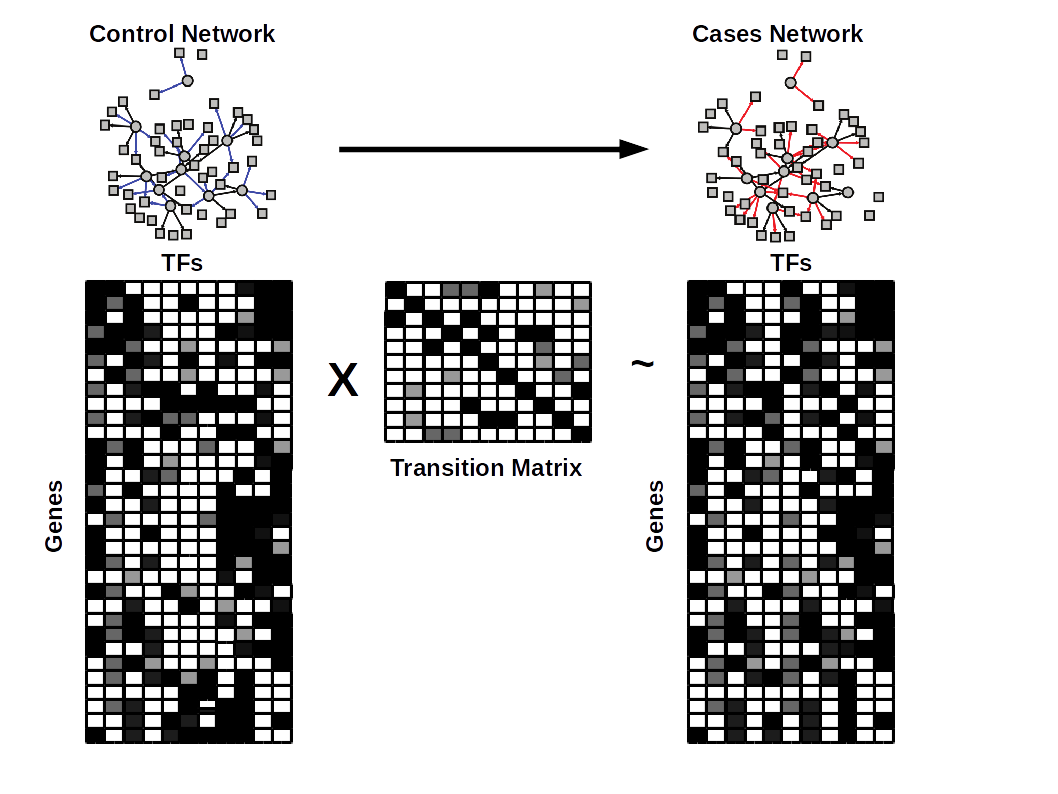
\includegraphics[width=0.5\columnwidth]{figure1}\caption{\textbf{Overview of the Transition Matrix problem.} Our approach seeks
to find the $TF\times TF$ matrix which best characterizes the transition
in TF targetting between cases and controls. We can think about this
problem as the estimation of the set of TF-TF interactions which minimizes
edgeweight error in the cases network when applied to the controls
network.}
\end{figure}


While it is appealing to conceive of this process as deterministic,
reflecting a change from one well-defined phenotype to another, in
truth the situation is much more complex. Neither the initial nor
the final phenotype is discrete, but each falls into a continuum of
states, which, on average, captures the features of that phenotype.
Indeed, within each tissue there are many, many cells, each of which
is its own particular instance of that tissue—with unique patterns
of gene expression and individual regulatory processes. In the language
of adjacency matrices, what this means is that rather than representing
each state by a matrix with binary entries, what one should do is
use a representation in which entries are continuous, representing
the strength of the transcription factor-target gene interaction averaged
over the collection of samples (or cells) representing each state.
And consequently, the problem of estimating the transition matrix
is generalized to solving , where E is an $m\times n$ error matrix
representing the uncertainty in the estimation of the individual edges.
In this formalism, modeling the cell state transition is equivalent
to estimating the appropriate transition matrix T that maps how the
transcription factor-target gene interactions are “rewired” between
states. And one could hypothesize that the drivers of the cell state
transition are those transcription factors that are have the greatest
change in the targets that they regulate. In evaluating the state
transitions, we recognize the limitations of current network inference
methods to predict individual edgeweights. It's therefore of interest
to combine measurements across sets of edgeweights in order to extract
meaningful signal from a network perturbation. Effectively, we approached
the problem as a dimension reduction problem with the goal of identifying
high-influence systematic regulatory network alterations rather than
isolated independent events. There are many existing methods for reducing
a high-dimensional matrix such as a gene regulatory adjacency matrix.
Commonly, Principal Components Analysis (PCA) identifies eigenvectors
which can reconstruct the greatest degree of variance from the original
data. One drawback of this approach is the lack of interpret-ability
of these vectors. Our transition matrix approach can be considered
as a data reduction method which (1) preserves the intuitive interpretation
of its vectors and (2) utilizes our expectation that meaningful network
transitions will occur via biologically systematic alterations and
not via random, independent edge alterations. 


\section*{TM significantly improves TF-TF edge estimation from simulated gene
expression data }

To evaluate the ability of our method to recover edges between transcription
factors, we generated simulated gene expression data. We began by
generating a true controls adjacency matrix, $M_{0\left(p\times q\right)}$,
describing the weighted edges between $q$ transcription factors and
$p$ genes. A state transition was generated by sampling 100 TF-TF
pairs and adjusting the edgeweight at the corresponding point on the
true cases adjacency matrix, $M_{1\left(p\times q\right)}$. These
TF-TF pairs ultimately represent the edges that we seek to recover
and the size of the adjustments are the parameters of interest. We
sampled from a multivariate Gaussian distribution with the off-diagonal
of the variance-covariance matrix, $\Sigma$, defined as the $M_{0}M_{0}^{\prime}$.
Furthermore, we scaled the magnitude of the diagonal of $\Sigma$
to achieve the desired proportion of noise. We aimed for an area under
the curve of the receiver-operator characteristic of approximately
0.70 as this has reasonably been achieved in existing biological studies~\cite{glass2013passing}. 

This sampling represented our simulated control samples. The adjusted
adjacency matrix, $M_{1}$, was similarly used to generate simulated
expression data for the cases group. Next, we reconstructed the networks
from our expression data using a set of commonly used network inference
methods - Weighted Gene Correlation Network Analysis (WGCNA)~\cite{Langfelder2008WGCNA}~\cite{Langfelder2008FastR},
Topological Overlap Measure (TOM)~\cite{ravasz2002hierarchical},
Algorithm for the Reconstruction of Gene Regulatory Networks (ARACNE)~\cite{margolin2006aracne},
Context Likelihood of Relatedness (CLR)~\cite{faith2007large}, Passing
Attributes between Networks for Data Assimilation (PANDA)~\cite{glass2013passing}
and simple Pearson correlation (PC). 

We applied the transition matrix with default parameters on each case-control
pair of networks. For comparison, we estimated the difference from
case to control in edgeweights derived from the direct edge prediction
using each network inference method. The predictions for the TM approach
and the direct approach were evaluated by the area-under-the-curve
of the receiver-operator-characteristic (AUCROC) with the true transition
adjustments taken as the gold standard. For each of the network inference
methods tested, we found substantial improvement in the predicted
transitions over the direct network inference method. In many cases,
the edgeweight difference (column 2) was not statistically significant
for predicting transitions, but when the TM was applied (column 3)
a strong predictive signal appeared. In other cases, an existing signal
was observed using the direct approach, but was dramatically improved
with the application of the TM.

The intuition behind the improvement is simple. While the estimation
of a TF-TF edge is typically evaluated via some pairwise gene expression
pattern which may be rife with technical and biological noise, the
TM approach borrows information from all downstream targets in estimating
the relative change in relationship between the TFs. 

{\tiny

\begin{table}
\begin{tabular}{|cc||c|c|}
\multicolumn{4}{c}{AUC-ROC for Eedgeweight differences vs Transition Matrix using various
NI methods}\tabularnewline
\hline 
\multirow{2}{*}{\textbf{NI Method}} & \multirow{2}{*}{\textbf{Networks}} & \textbf{Edgeweight } & \textbf{Transition}\tabularnewline
 &  & \textbf{differences} & \textbf{Matrix}\tabularnewline
\hline 
Pearson & .701 (p<.0001) & .510 (p=.72) & .802 (p<.0001)\tabularnewline
\hline 
WGCNA(6) & .701 (p<.0001) & .512 (p=.61) & .688 (p<.0001)\tabularnewline
\hline 
WGCNA(12) & .701 (p<.0001) & .52 (p=.10) & .589 (p=.02)\tabularnewline
\hline 
ARACNE & .515 (p<.0001) & .523 (p=.58) & .566 (p=.09)\tabularnewline
\hline 
CLR & .691 (p<.0001) & .57 (p=.19) & .814 (p<.0001)\tabularnewline
\hline 
TOM & .700 (p<.0001) & .51 (p=.62) & .689 (p<.0001)\tabularnewline
\hline 
PANDA{*}(Motif=.570) & .740 (p<.0001) & .520 (p=.13) & .793 (p<.0001)\tabularnewline
\hline 
PANDA{*}{*} (Motif=.547) & .676 (p<.0001) & .509 (p=.43)  & .66 (p<.0001) \tabularnewline
\hline 
\end{tabular}\caption{\textbf{Comparison of edgeweight difference to Transition Matrix in
simulated case-control gene expression}. Several network inference
methods were run on our \emph{in silico} case-control data. The overall
network area under the curve of the receiver-operator characteristic
(AUC-ROC) was performed for each method averaged across cases and
controls. For PANDA{*} and PANDA{*}{*}, which additionally utilizes
motif prior information, motif priors with AUC-ROC of .570 and .547
were used. The naive TF-TF transitions were calculated as the difference
in TF-TF edgeweight between cases and controls. The transition matrix
TF-TF transitions used the absolute transition matrix values. }
\end{table}


}


\section*{Transition Matrix Analysis}

Many mechanisms which may be differentially present, such as RNA degredation,
post-translational modification, protein-level interactions and epigenetic
alterations have the ability to impact downstream targeting without
impacting the expression level of the TF itself. It may be of particular
scientific or therapeutic interest to identify those TFs which have
undergone significant overall changes in behavior between controls
and cases. With that objective in mind, we express the statistic-
differential Transcription Factor Involvement (DTFI), as a measure
for quantifying this property. 
\[
s_{j}=\frac{\sum_{i=1}^{m}I\left(i\ne j\right)\tau_{i,j}^{2}}{\sum_{i=1}^{m}\tau_{i,j}^{2}}
\]
 DTFI can be loosely interpreted as the proportion of TF targeting
patterns which is explained by the targeting patterns of other available
TFs. This measure, a statistic on the interval $[0,1]$ seeks to elucidate
transitions which are systematic, informative, and non-arbitrary in
nature by capturing only the edgeweight signal for which there is
an attributable regulatory pattern. The distribution of this statistic
under the null has a mean and standard deviation which depend on the
motif structure. In particular, both mean and standard deviation are
increased for TFs which have fewer prior regulatory targets. From
a statistical perspective, TFs with relatively more targets are able
to generate more stable targeted expression patterns, which leads
to more consistent estimates in “agreement” algorithms such as PANDA
and BERE. From a biological perspective, increased motif presence
may indicate that the TFs are more likely to be ubiquitous housekeeping
proteins that do not meaningfully alter their involvement between
cases and controls. The dependence of the null distribution on the
motif structure is addressed via the following resampling procedure. 
\begin{enumerate}
\item Gene expression samples are randomly assigned to case and control
forming the null-case and null-control with group sizes preserved. 
\item GRNs are reconstructed for the null-case and null-control with the
same prior regulatory structure. 
\item The transition matrix algorithm is applied for the two null networks. 
\item The differential TFI is calculated for each TF. 
\item Repeat 1-4 1000 times. 
\end{enumerate}
\begin{figure}
\begin{centering}
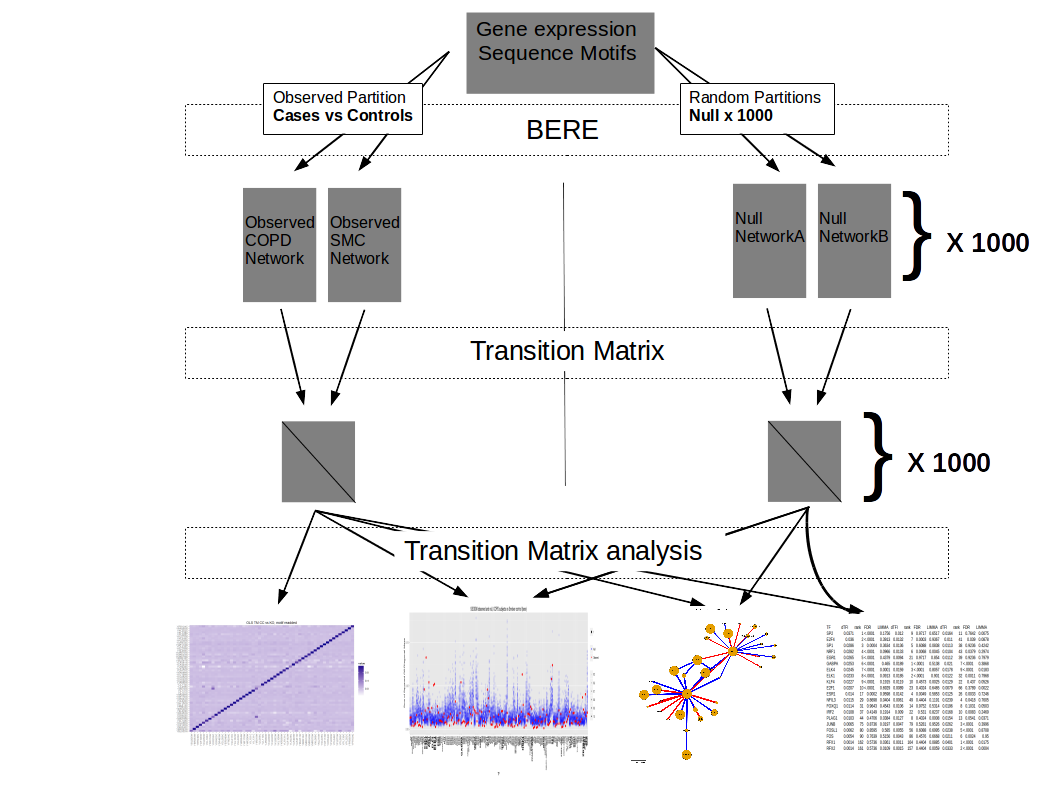
\includegraphics[width=0.8\columnwidth]{workflow_diagram}\caption{\textbf{Overview of Transition Matrix analysis workflow.} (1) BERE
is applied separately to subsets of the gene expression data including
the cases group, the controls group and 1000 permutations of the cases
and controls labels. (2) Transition matrix is estimated between the
cases and controls and each of the pair or permuted ``cases'' and
``controls''.}

\par\end{centering}

\end{figure}



\section*{Transition Matrix finds concordance in independent datasets for COPD }

We applied our method to three case-control datasets for Chronic Obstructive
Pulmonary Disease (COPD)- Evaluation of COPD Longitudinally to Identify
Predictive Surrogate Endpoints (ECLIPSE), the COPDGene study, and
Lung Genomics Research Consortium (LGRC). Each of these studies consisted
of gene expression assays obtained from patients with COPD and a set
of smoker controls. The tissue used in the ECLIPSE and COPDGene study
was peripheral blood mononuclear cell (PBMC), while lung tissue was
sampled for LGRC. It is therefore unsurprising that agreement is more
strongly achieved in the former studies compared to the latter. However
it is quite notable that the we do see much of the same dTFI signal
across studies involving different tissue types.

We separately applied our BERE network inference approach on cases
and controls and computed the transition matrix. Top significance
hits for dTFI showed strong concordance between each of the datasets.
Out of 166 TF used in this study, seven were among top 10 most differentially
involved in both the ECLIPSE and COPDGene studies. Furthermore, three
of these seven TFs (GABPA, ELK4, ELK1) also appeared as significant
in the LGRC results with FDR<.01. 

Overall, there was a strong correlation between results in the two
PBMC studies $\left(R^{2}=0.82\right)$, and a weak correlation between
cross-tissue results for LGRC-ECLIPSE $\left(R^{2}=0.33\right)$ and
LGRC-COPDGene$\left(R^{2}=0.39\right)$.
\begin{figure}[h]
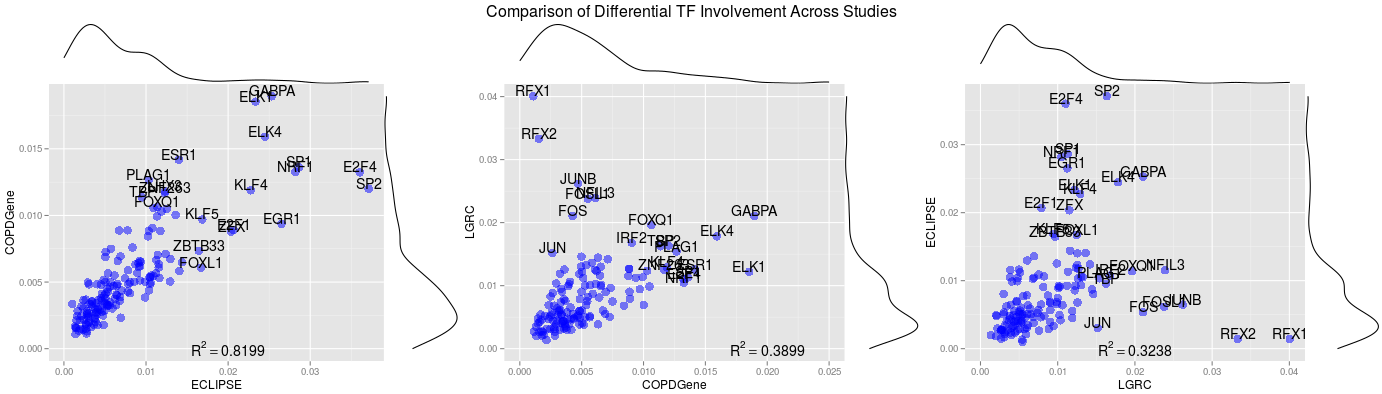
\includegraphics[width=1\columnwidth]{pasted12a}

\caption{Comparison of dTFI for 166 TFs across three independent studies. Results
for two studies with gene expression data obtained from PBMC (ECLIPSE
and COPGene) show strong concordance with a high degree of agreement,
particularly for top hits. Both of these studies are less consistent
with the LGRC, but contain several significant TFs in agreement with
the other studies.}


\end{figure}


Of further interest is the particular TFs which are differentially
observed across studies. For example, ERS1, the gene encoding Estrogen
receptor alpha (ES-$\alpha$) is likely to behave differently in males
compared with females. We found that this TF is significantly differentially
involved in the COPDGene study - identified as the $4th$ most differentially
involved TF, but not the ECLIPSE study. Accordingly, the COPDGene
study had a greater gender disparity $\left(\mbox{Odds Ratio}=1.126\right)$
than the ECLIPSE study $\left(\mbox{Odds Ratio}=1.067\right)$.

Notably in the LGRC dataset, we discovered a differential targetting
pattern involving the TFs RFX1 and RFX2. Both of these transcription
factors were highly statistically significant (FDR<.0001) and ranked
as the top two results in the LGRC study. However, their signal was
muted in the ECLIPSE and COPDGene studies, neither of which identified
these transcription factors as drivers of the Smoker Control to COPD
transition. There are many possible explanations for this result,
but it is reasonable to speculate that the dramatically different
result is due to the fact that the tissue of origin for the LGRC differs
from the ECLIPSE and COPDGene tissue.

The top hits which are most consistent across studies have been implicated
in independent studies for the development of COPD.

Two of the top 3 hits, NRF1 and GABPA have been implicated in a mitochondrial
mechanism for disease progression {[}Cloonan, Suzanne M et al{]}.
Interestingly, the majority of the TFs identified as differentially
involved do not exhibit significant differential gene expression.
This suggests that for these proteins, their role in the disease may
not occur until the post-transcription stage. It also suggests that
conventional gene expression analysis is insufficient for identifying
many of the TF drivers of disease.

\begin{table}
{\center {\tiny

\begin{tabular}{|c||c|c|c|c||c|c|c|c||c|c|c|c|}
\hline 
 & \multicolumn{4}{c||}{ECLIPSE} & \multicolumn{4}{c||}{COPDGene} & \multicolumn{4}{c|}{LGRC}\tabularnewline
\hline 
TF & dTFI & rank & FDR & LIMMA & dTFI & rank & FDR & LIMMA & dTFI & rank & FDR & LIMMA\tabularnewline
\hline 
\hline 
SP2 & .0371 &   1 & <.0001 & .1756 & .0120 &   9 & .9717 & .6517 & .0164 & 11 & .7642 & .0075\tabularnewline
\hline 
E2F4 & .0360 &   2 & <.0001 & .3913 & .0132 &   7 & .0003 & .9367 & .0110 & 41 & .039 & .0878\tabularnewline
\hline 
SP1 & .0286 &   3 & .0004 & .3634 & .0136 &   5 & .6088 & .0838 & .0113 & 38 & .9236 & .4242\tabularnewline
\hline 
NRF1 & .0282 &   4 & <.0001 & .0966 & .0133 &   6 & .0068 & .0045 & .0104 & 43 & .0379 & .2974\tabularnewline
\hline 
EGR1 & .0265 &   5 & <.0001 & .4379 & .0094 &  21 & .9717 & .8540 & .0112 & 39 & .9236 & .7979\tabularnewline
\hline 
GABPA & .0253 &   6 & <.0001 & .4650 & .0189 &   1 & <.0001 & .5138 & .0210 &  7 & <.0001 & .3868\tabularnewline
\hline 
ELK4 & .0245 &   7 & <.0001 & .0001 & .0159 &   3 & <.0001 & .8057 & .0178 &  9 & <.0001 & .0183\tabularnewline
\hline 
ELK1 & .0233 &   8 & <.0001 & .0913 & .0185 &   2 & <.0001 & .9010 & .0122 & 32 & .0011 & .7968\tabularnewline
\hline 
KLF4 & .0227 &   9 & <.0001 & .1915 & .0119 &  10 & .4573 & .0025 & .0129 & 22 & .437 & .0526\tabularnewline
\hline 
E2F1 & .0207 &  10 & <.0001 & .6929 & .0089 &  23 & .4024 & .6465 & .0079 & 66 & .3789 & .0022\tabularnewline
\hline 
ESR1 & .0140 &  17 & .0002 & .9598 & .0142 &   4 & .0049 & .5853 & .0125 & 26 & .0033 & .7246\tabularnewline
\hline 
NFIL3 & .0115 &  29 & .8698 & .0404 & .0061 &  49 & .4404 & .1191 & .0239 &  4 & .0418 & .7605\tabularnewline
\hline 
FOXQ1 & .0114 &  31 & .9643 & .4543 & .0106 &  14 & .9752 & .5314 & .0196 &  8 & .1031 & .0503\tabularnewline
\hline 
IRF2 & .0108 &  37 & .4149 & .1914 & .0090 &  22 & .531 & .8237 & .0168 & 10 & .0083 & .2469\tabularnewline
\hline 
PLAG1 & .0103 &  44 & .4706 & .0384 & .0127 &   8 & .4024 & .0008 & .0154 & 13 & .0541 & .0371\tabularnewline
\hline 
JUNB & .0065 &  75 & .8736 & .0197 & .0047 &  79 & .5281 & .9526 & .0262 &  3 & <.0001 & .3996\tabularnewline
\hline 
FOSL1 & .0062 &  80 & .8595 & .5850 & .0055 &  56 & .6088 & .6995 & .0238 &  5 & <.0001 & .8708\tabularnewline
\hline 
FOS & .0054 &  90 & .7639 & .5156 & .0043 &  86 & .4576 & .6668 & .0211 &  6 & .0024 & .9500\tabularnewline
\hline 
RFX1 & .0014 & 162 & .5736 & .0361 & .0011 & 164 & .4404 & .0885 & .0401 &  1 & <.0001 & .0175\tabularnewline
\hline 
RFX2 & .0014 & 161 & .5736 & .0109 & .0015 & 157 & .4404 & .0059 & .0333 &  2 & <.0001 & .0004\tabularnewline
\hline 
\end{tabular}}}\caption{Combined list of TFs which were among the top 10 hits (out of 166
available TFs) in any of the 3 studies, ordered by the dTFI in the
ECLIPSE study. For each study, columns indicate the TF's (1) differential
TF Involvement, (2) dTFI Rank within list of TFs, (3) Significance
of dTFI by false discovery rate, and (4) p-value for LIMMA differential
gene expression analysis.}
\end{table}


\begin{figure}[h]
\textbf{A}

\textbf{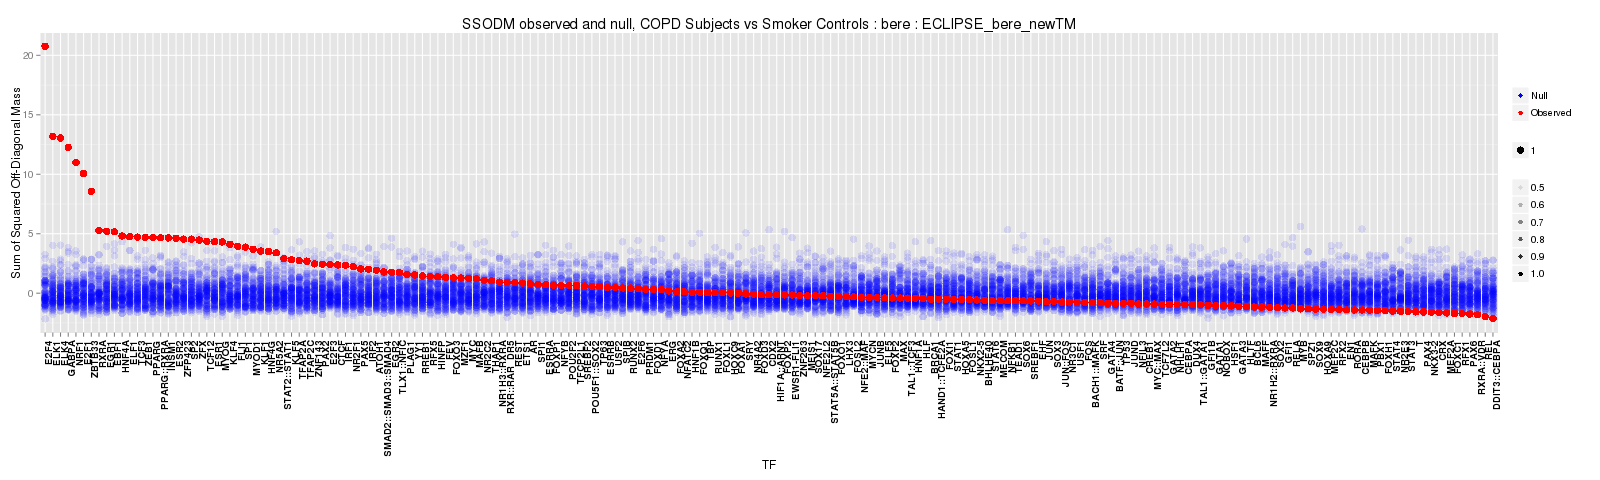
\includegraphics[width=1\columnwidth]{pasted6a}}

\textbf{B}

\textbf{\includegraphics[width=1\columnwidth]{\string"dTFI vs LIMMA55557\string".png}}

\textbf{C}

\includegraphics[width=0.5\columnwidth]{\string"Transition plot55557\string".png}

\caption{\textbf{(A)} Differential transcription factor involvement for the
observed case-control (red) scaled for each TF by the distribution
under the randomized case-control. \textbf{(B) Comparison of TF differential
involvement vs differential expression.} TFs which are differentially
involved are not necessarily differentially expressed and vice versa.
Many TFs can be observed which have significantly different targetting
patterns, but which are not statistically significantly differentially
expressed. This suggests that our method finds transcription factors
which are differentially affected at a post-transcription stage. \textbf{(C)
Driver network transitions}. Network transitions are depicted here
with arrows indicating the flow of targetting patterns from one transcription
factor to another. Edges are sized according to the magnitude of the
transition and nodes (TFs) are sized by the overall dTFI for each
TF. The gain of targetting features is indicated by the color blue
while the loss of features is indicated by red.}
\end{figure}



\part*{Supplement}

The computations in this paper were run on the Odyssey cluster supported
by the FAS Division of Science, Research Computing Group at Harvard
University.


\section*{Transition matrix finds significant protein-protein interaction}

As noted above, there are numerous biological regulatory mechanisms
which may yield detectable transitions. Of particular interest are
those which are less readily detectable via conventional methods,
such as differential gene expression analysis. One mechanism studied
here involves one TF binding to another TF to promote, suppress or
alter one or both of their regulatory patterns. These multi-protein
interactions create combinatorial complexity that can explain much
of the variation in organism complexity which is unexplained by number
of genes alone~\cite{levine2003transcription}.

To test the ability to detect protein level interactions, we compared
our estimated transitions to a set of known protein-protein interactions
\cite{ravasi2010atlas}. This set contained 223 pairwise interactions
between a total of 189 transcription factors. Of interest was the
effectiveness of identifying these interactions via the transition
from one phenotypic state to another. This is a challenging task for
several reasons, (1) protein-protein interaction is merely one of
a myraid of detectable transition mechanisms, (2) it is reasonable
to assume that only a small subset of the known PPI are actually differentially
present between case and control and (3) technological limitations
in the active field of proteomics cannot be expected to identify all
interactions with a reasonable degree of certainty.

For the transition from Smoker control to COPD, we compared for the
transition estimates to those generated by the transition from randomly
resampling the phenotypic labels. The AUCROC for the prediction of
the 223 known protein-protein interactions was $0.5695\left(p=0.018\right)$,
suggesting that our approach is successful at detecting this highly
obscured signal.
\begin{figure}[h]
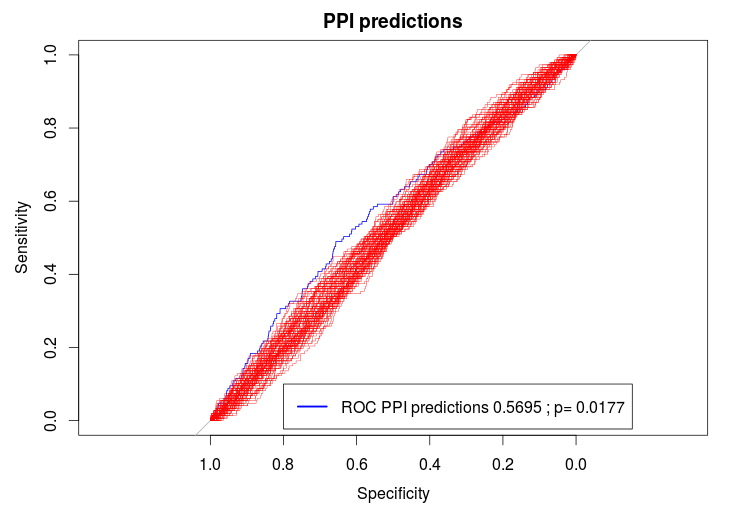
\includegraphics[width=0.5\columnwidth]{pasted9a}\caption{ROC curve for prediction of PPI based on a transition from Smoker
control to COPD (blue) compared to a random case-control partition
of the ECLIPSE data.}
\end{figure}



\section*{Efficiency of estimation}

Let $\mathbf{x}_{p}$ be a Gaussian $p$-vector representing a sample
of gene expression data containing $q$ transcription factors and
$p-q$ non-transcription factor genes. 
\[
\mathbf{x}_{p}\sim N\left(\mathbf{\mu},\Sigma\right)
\]
where $\mathbf{\mu}$ is the $p$-vector of mean gene expression values
and $\Sigma$ is the $p\times p$ variance-covariance matrix. In this
scenario, $\Sigma$ may be regarded as a combination of two independent
variance-covariance sources- (1) biological signal, (2) biological
noise and technical noise.

In investigating gene regulation, many network inference methods are
constructed for the estimation of the $p\times q$ subset of $\Sigma$
pertaining to the effect of the $q$ TFs on the $p$ genes. In identifying
drivers of state transitions, we seek to focus on the $q\times q$
matrix of TF-TF effects. We show that our method vastly ourperforms
commonly used network inference methods in estimating these specific
effects.

Consider a state change between two experimental conditions, A and
B, characterized by an alteration of size $\delta$ to the biological
signal component of the TF-TF variance-covariance matrix at point
$\Sigma_{i,j}$ where $i$ and $j$ are indices for two TFs in $\Sigma$.

Using a univariate coexpression calculation (the basis for Pearson
networks and WGCNA estimates), the estimated variance of our estimate
of $\delta$ can be calculated:

\[
-\rho_{A}<\delta<\rho_{A},\delta+\rho_{A}\le1
\]


\begin{eqnarray*}
Var\left(\hat{\rho}_{i,j,A}-\hat{\rho}_{i,j,B}\right) & = & Var\left(\hat{\delta}_{cor}\right)\\
 &  & Var\left(\hat{\rho}_{i,j,A}\right)+Var\left(\hat{\rho}_{i,j,B}\right)\\
 & = & \frac{1-\rho_{i,j,A}^{2}}{n_{A}-2}+\frac{1-\rho_{i,j,B}^{2}}{n_{B}-2}\\
 & = & \frac{1}{n_{A}-2}+\frac{1}{n_{B}-2}-\frac{\rho_{i,j,A}^{2}}{n_{A}-2}-\frac{\rho_{i,j,B}^{2}}{n_{B}-2}
\end{eqnarray*}
Meanwhile, in condition B the new correlation of $TF_{i}$ with some
gene, $gene_{k}$ $k\in1,2\dots p$ , denoted $cor^{*}$, becomes
\[
cor^{*}\left(TF_{i},gene_{k}\right)=cor\left(TF_{i},gene_{k}\right)+\delta cor\left(TF_{j},gene_{k}\right)
\]
where the term $\delta cor\left(TF_{j},gene_{k}\right)$ is the change
due to the interaction of $TF_{i}$ and $TF_{j}$. 

The variance of our estimate using the transition matrix can be expressed
as follows:
\begin{eqnarray*}
Var\left(TM_{i,j}\right) & = & Var\left(\hat{\delta}_{TM}\right)\\
 & = & \frac{\left(\frac{1}{p}\right)\sum_{k=1}^{p}vVar\left(\hat{\rho}_{i,k,A}-\hat{\rho}_{i,k,B}\right)}{\sum_{k=1}^{p}\left(\rho_{j,k}-\bar{\rho_{j}}\right)^{2}}\\
\\
 & = & \frac{\left(\frac{1}{p}\right)\sum_{k=1}^{p}\left[Var\left(\hat{\rho}_{i,k,A}\right)+Var\left(\hat{\rho}_{i,k,B}\right)\right]}{\sum_{k=1}^{p}\left(\rho_{j,k}-\bar{\rho_{i}}\right)^{2}}\\
 & \le & \frac{\left(\frac{1}{p}\right)\sum_{k=1}^{p}\left[\frac{1}{n_{A}-2}+\frac{1}{n_{B}-2}\right]}{\sum_{k=1}^{p}\left(\rho_{j,k}-\bar{\rho_{i}}\right)^{2}}\\
 & \le & \frac{\frac{1}{n_{A}-2}+\frac{1}{n_{B}-2}}{\sum_{k=1}^{p}\left(\rho_{j,k}-\bar{\rho_{i}}\right)^{2}}\\
 & \le & \frac{Var\left(\hat{\delta}_{cor}\right)+\frac{\rho_{i,j,A}^{2}}{n_{A}-2}+\frac{\rho_{i,j,B}^{2}}{n_{B}-2}}{\sum_{k=1}^{p}\left(\rho_{j,k}-\bar{\rho_{i}}\right)^{2}}\\
 & \le & Var\left(\hat{\delta}_{cor}\right)+\frac{Var\left(\hat{\delta}_{cor}\right)\left(1-\sum_{k=1}^{p}\left(\rho_{j,k}-\bar{\rho_{i}}\right)^{2}\right)+\frac{\rho_{i,j,A}^{2}}{n_{A}-2}+\frac{\rho_{i,j,B}^{2}}{n_{B}-2}}{\sum_{k=1}^{p}\left(\rho_{j,k}-\bar{\rho_{i}}\right)^{2}}
\end{eqnarray*}
So we have that $Var\left(TM_{i,j}\right)<Var\left(\hat{\delta}_{cor}\right)$
when
\[
Var\left(\hat{\delta}_{cor}\right)\left(1-\sum_{k=1}^{p}\left(\rho_{j,k}-\bar{\rho_{i}}\right)^{2}\right)<\frac{\rho_{i,j,A}^{2}}{n_{A}-2}+\frac{\rho_{i,j,B}^{2}}{n_{B}-2}
\]
Since each term except $\left(1-\sum_{k=1}^{p}\left(\rho_{j,k}-\bar{\rho_{i}}\right)^{2}\right)$
is strictly non-negative, we see that this inequality holds when 
\[
\sum_{k=1}^{p}\left(\rho_{j,k}-\bar{\rho_{i}}\right)^{2}<1
\]
Thus, we have a more efficient estimator of $\delta$ when 
\[
p>\frac{1}{Var\left(\rho_{j,k}\right)}
\]
In practice, we typically have a large number of genes, $p$, so that
our transition matrix estimator will be expected to be dramatically
more efficient than the commonly used Pearson or WGCNA estimators.

\bibliographystyle{plain}
\bibliography{dissertation_research}

\end{document}
